\documentclass[a4paper,twoside]{article}

\usepackage{epsfig}
\usepackage{subcaption}
\usepackage{calc}
\usepackage{amsfonts}
\usepackage{amssymb}
\usepackage{amstext}
\usepackage{amsmath}
\usepackage{amsthm}
\usepackage{array}
\usepackage{cite}
\usepackage{enumitem}
\usepackage{graphicx}
\usepackage{hyperref}
\usepackage{multicol}
\usepackage{pslatex}
\usepackage{algorithm2e}
\usepackage{xcolor}

\usepackage[font=scriptsize]{caption}
\usepackage[bottom]{footmisc}

\usepackage{SCITEPRESS}     % Please add other packages that you may need BEFORE the SCITEPRESS.sty package.


\graphicspath{ {./img/} }

% Document
\begin{document}
    \title{PyResolveMetrics: A Standards-Compliant and Efficient Approach to Entity Resolution Metrics}
    \author{\authorname{Andrei Olar\sup{1}\orcidAuthor{0009-0006-7913-9276}}
    \affiliation{\sup{1}Faculty of Computer Science, Babes-Bolyai University}
    \email{\{andrei.olar\}@ubbcluj.ro}
    }
    \keywords{Entity Resolution,Metrics,Library,Open Source,Standards-Compliant,Theoretical Model,Efficiency}

    \abstract{Entity resolution, the process of discerning whether multiple data
    refer to the same real-world entity, is crucial across various domains.
    Its quality assessment is increasingly vital due to the extensive practical
    applications in fields such as natural language processing, information
    retrieval, and machine learning.
    With Python emerging as the predominant programming language in these areas,
    this paper attempts to fill in a gap when evaluating the qualitative
    performance of entity resolution tasks by proposing a novel consistent
    library dedicated exclusively for this purpose.
    This library not only facilitates precise evaluation but also aligns with
    contemporary research and application trends, making it a significant tool
    for practitioners and researchers in the field.}

    \onecolumn \maketitle \normalsize \setcounter{footnote}{0} \vfill

    \section{Introduction}\label{sec:introduction}
    Entity resolution involves determining whether two pieces of information
    represent the same real-world item.
    Some definitions view it as identifying and linking data from multiple
    sources\cite{Qia17}.
    However, it's argued that this identification and linking is a more
    specialized process\cite{Tal11}.
    Entity resolution, a broad issue, is known by various names including record
    linkage, data deduplication, merge-purge, named entity recognition, entity
    alignment, and entity matching.

    Entity resolution has many practical applications ranging from linking
    medical records to diagnosing diseases or ailments, to doing background
    checks to detect financial crime or to identifying plagiarism.
    Being a problem whose solutions could have a deep impact on both individual
    well-being and human society, we are obviously interested in understanding
    just how well entity resolution solutions fare.
    This paper attempts to address that issue by introducing a new library that
    provides implementations of some of the best known metrics for evaluating
    entity resolution\cite{matchescu-er-metrics2023}.

    In the book ``Introduction to Information Retrieval'' we are acquainted with
    a number of ways in which the performance of information retrieval systems
    can be evaluated\cite{manning2008}.
    The metrics presented in this book revolve around the notion of relevant and
    irrelevant information that is retrieved by the system.
    The book also clarifies that the judgement around what is relevant or not is
    stipulated in a golden standard or a ground truth.
    Furthermore, this golden standard is dependant upon an information need.

    Entity resolution systems partly function as information retrieval systems,
    as they determine whether multiple data points refer to the same real-world
    entity.
    This capability to discern data identity within a context is the fundamental
    information need of any entity resolution system.
    Is it therefore fitting to use information retrieval metrics for entity
    resolution?
    This seems to be the consensus drawn in the scientific literature as we
    shall see in the next section.

    The library we are introducing implements various information retrieval
    metrics adapted for entity resolution.
    It's also important to acknowledge the distinct mathematical models
    underlying entity resolution compared to information retrieval.
    The library sets itself apart by organizing metrics based on their
    compatibility with entity resolution models, influenced by the underlying
    differences in data structures that are characteristic to each model.
    Special attention is given to interoperability and the seamless integration
    of the library into the Python programming language ecosystem.

    In short, we present a library that has the following key features:

    \begin{enumerate}
        \item embracing an OpenSource licensing model,
        \item efficient implementation using state of the art libraries under
        a very popular platform, and
        \item a design that is agnostic to the entity resolution implementation.
    \end{enumerate} 

    The outline of this article is as follows.
    After this introduction, we overview two existing mathematical models for
    entity resolution which, in spite of their age, are still widely used and
    still represent the state of the art.
    Then we go through other work that relates to this paper.
    Subsequently, we present the new library and pay special attention to the
    reasons for implementing it.
    We go over the metrics that are implemented, the technological and design
    choices that were made, an example of using the library and a performance
    evaluation of the functions implemented by the library.
    In the end we offer some conclusions and present aspects that require more
    work.

    \section{Entity Resolution Models}\label{sec:models}
    \subsection{Fellegi-Sunter Model}
    In the late 1960s Ivan Fellegi and Alan Sunter wrote the seminal
    paper\cite{fs1969} for what they called record linkage and what would later
    become known as entity resolution.
    To this day, their mathematical model based on probability theory is the
    most popular way of formalizing the entity resolution problem.
    In this mathematical model, entity resolution is a function that aids in 
    probabilistic decision making.
    
    In this model of entity resolution, the process primarily involves comparing
    data from two sources.
    The essential step is matching two items --- one from each source, after
    which a decision is made to categorize the match as a `link', `non-link', or
    `possible link'.
    Consequently, any matching algorithm under this model typically returns
    pairs of items from the original data sources, each tagged as one of these
    categories.
    However, in practical applications today, this process is often simplified
    to just returning a list of pairs labeled as `links'.

    This intuitive explanation gives us the structure of the input we can expect
    when we use the Fellegi-Sunter entity resolution model: an iterable sequence
    of pairs.

    The metrics that are implemented with the Fellegi-Sunter model of entity
    resolution in mind will accept iterable sequences of pairs as input where
    the ground truth and the result of the entity resolution task are concerned.

    \subsection{Algebraic Model}
    The algebraic model for entity resolution, initially conceived for assessing
    information quality in large datasets\cite{tal2007algebraic}, was later
    refined to describe the entity resolution process itself\cite{Tal11}.
    This model treats entity resolution as an algebraic equivalence relation
    over a given input set, which can include data from as many original sources
    as necessary.
    
    The unique aspect of this model lies in the characteristics of equivalence
    relations\cite{halmos1960naive}.
    These relations create partitions over the input set, with each partition
    component equivalent to an equivalence class of the relation\cite{Tal11}.
    Conversely, a partition over a set can also induce an equivalence relation.

    With this in mind, evaluating the outcome of an entity resolution task
    becomes as easy as comparing two partitions: the partition that induces the
    ideal equivalence relation (the gold standard or ground truth) to the
    partition that is produced by the entity resolution task.
    The library supports a few metrics for comparing partitions, all of which
    expect that a partition is represented as a list of sets.

    \section{Related Work}\label{sec:related}

    Measuring entity resolution quality was a subject of interest ever since the
    first paper on the subject surfaced\cite{newcombe1959}.
    The paper speaks about accuracy and contamination similarly to the current
    notions of true and false positives.
    The fundamental theory of record linkage\cite{fs1969} offers a probabilistic
    approach to evaluating the success of an entity resolution task.
    It suggests methods to affect the results through the selection of suitable
    thresholds for defining success and failure.
    It also provides mechanisms for properly weighting for independent
    probability variables.
    The literature expands on these techniques in subsequent
    papers\cite{winkler1990}.
    Some of the entity resolution evaluation metrics that are a direct result of
    this theoretical foundation include match accuracy, match
    rate\cite{jaro1989advances}, error rate estimation, rate of clerical
    disambiguation\cite{winkler1990} or relative distinguishing
    power of matching variables\cite{winkler2014}.
    A good amount of effort is spent on estimating and measuring the
    effectiveness of blocking techniques to reduce the input size of the data
    set used for evaluation purposes\cite{winkler1990,jaro1989advances}.
    Measuring entity resolution performance was and remains a computationally
    intensive task.
    
    Concerns about using accuracy and match rate are also voiced\cite{Goga2015}.
    Thus we see a shift towards metrics used in the related field of information
    retrieval.
    The probabilistic model for entity resolution aligns well with concepts such
    as true/false positives/negatives.
    Given the extensive history of using ground truths to assess entity
    resolution quality, there is a natural fit for using information retrieval
    quality metrics.
    Most literature on this topic focuses on using information retrieval metrics
    where the order in which results are retrieved is not
    relevant\cite{manning2008}.

    Besides the original statistical model for entity resolution, other models
    have evolved from it or alongside it.
    The work of the InfoLab at Stanford on their Stanford Entity Resolution
    Framework\cite{Ben2009Swoosh} and that of the Center for Entity Resolution
    and Information Quality at the University of Arkansas in Little
    Rock\cite{tal2007algebraic} stand out.
    These models of entity resolution also propose new metrics for evaluating
    entity resolution quality\cite{Men10,Tal11}.

    Also related to this paper, there is ample coverage of the metrics used for
    entity resolution in syntheses on the subject\cite{vldb2010,hitesh2012,Tal11}.
    Metrics that measure aspects of clustering seem to be used more frequently
    to measure entity resolution quality as time passes.
    For example, pairwise and cluster metrics\cite{Men10, huang2006efficient} or
    the Rand index\cite{tal2007algebraic} come up regularly in this context.

    Lastly, there are numerous systems that perform entity resolution available.
    Some of these systems include modules to evaluate the performance of a
    particular entity resolution solution\cite{fever2009,magellan2020,oyster2012}.
    There are also other Python packages that implement some or all of the
    metrics provided by our library\cite{nmeth2020scipy,ereval}.

    \section{PyResolveMetrics}\label{sec:library}

    In this context, the necessity for yet another specialized library dedicated
    to evaluating entity resolution metrics might seem redundant.
    This skepticism is rooted in the expectation that Python, being a highly
    popular programming platform, should already offer high-quality, reusable
    tools available for a wide range of applications --- including evaluating
    entity resolution results.
    
    Upon closer examination of the tools available for evaluating entity
    resolution tasks, certain limitations in the existing assumptions become
    apparent.
    There are indeed numerous libraries offering packages for computing entity
    resolution metrics.
    However, using a general-purpose library like SciPy raises concerns about
    interoperability and efficiency.
    This is particularly relevant when the sole requirement is to compute entity
    resolution metrics, and the additional features of a comprehensive library
    are unnecessary.
    The challenge of seamlessly integrating entity resolution evaluation
    routines into a custom built project becomes even more pronounced when
    attempting to use the ones packaged with established entity resolution
    systems\cite{oyster2012,jedai2017,deepm2020,magellan2020}.
    
    Conversely, when specifically searching for libraries that only offer entity
    resolution metrics, it becomes evident that some crucial metrics essential
    for effectively evaluating entity resolution tasks may be absent\cite{ereval}.

    Approaching the issue from a different angle, using metrics from a
    general-purpose algorithmic library like Scipy (specifically
    \texttt{scipy.metrics}) for entity resolution evaluation requires strict
    adherence to certain design choices imposed by the library.
    For example, to calculate the Rand index, data clusters must be mapped with
    labels, and these labels must be provided as input.
    While this might seem simple, the user-friendliness of such an approach is
    debatable.
    The complexity of adapting existing data and managing the necessary labels
    for the package could potentially rival the complexity of computing the Rand
    index itself, mooting the use of the package.
    Furthermore, additional memory and compute time are also required to perform
    the mapping between own data structures and the ones required by the API
    contract.

    In short, here are the reasons we chose to implement such a library:
    \begin{itemize}
    \item Architecturally, adhering to the principle of 'do one thing and do
    it well' is beneficial.
    This approach avoids the biases and dependencies of general-purpose
    libraries like SciPy, which can complicate integration into our
    custom-designed software.
    \item Historically, entity resolution has adapted evaluation techniques from
    statistics, information retrieval, and graph theory, tailoring these methods
    to suit its specific needs.
    It seems desirable to standardize these methods into forms specific to
    entity resolution.
    \item Currently, there appears to be no implementation that consolidates all
    the metrics useful for entity resolution evaluation, as identified in
    scientific literature, into a single, cohesive unit.
    \item Our work has a significant component of evaluating entity resolution
    outcomes.
    \end{itemize}

    Our opinion is that using mathematical models specific to entity resolution
    is the best approach for guiding the library's design.
    Since each model significantly impacts the data structures used in
    evaluation, the library's functions are categorized based on the type of
    input they support and, implicitly, by the mathematical model they align
    with.

    There are a couple of important assumptions that the library makes,
    regardless of the entity resolution model.
    One such assumption is that the quality of the entity resolution output is
    always measured against a ground truth\cite{manning2008}.
    The other assumption is that the ground truth and the entity resolution
    result are both structured under the same mathematical model.

    \subsection{Supported Metrics}\label{sec:metrics}
    
    \subsubsection{Statistical Metrics}
    Statistical quality metrics, extensively detailed in the
    literature\cite{manning2008,hitesh2012}, are the most common method for
    measuring entity resolution performance as evidentiated by their almost
    ubiquitous usage\cite{fever2009,Goga2015,deepm2020,eager2021}.
    These metrics are linked to the Fellegi-Sunter model for entity resolution
    which provides clear definitions of Type I and Type II
    errors\cite{winkler1990}.
    Type I and Type II errors clarify the concepts of true positives, true
    negatives, false positives, and false negatives as they are used in entity
    resolution.
    Understanding these concepts necessitates referencing the $M$ (matches) and
    $U$ (non-matches) sets as defined in the seminal paper on the model.

    Depending on the expected location of a pair produced by the entity
    resolution function, we define:

    \begin{itemize}
        \item \textbf{true positives} as pairs predicted to be in $M$ that
        should be in $M$,
        \item \textbf{false positives}, or type I errors, as pairs predicted to
        be in $M$, but should be in $U$,
        \item \textbf{true negatives} as pairs predicted to be in $U$ that
        should be in $U$, and
        \item \textbf{false negatives}, or type II errors, as pairs predicted to
        be in $U$, but should be in $M$.
    \end{itemize}

    Several metrics based on these concepts exist, though the effectiveness of
    some has been questioned\cite{Goga2015}.
    With this in mind we finally define the three quality metrics that are
    supported by our library:

    \begin{align}
    Precision&=\frac{true\,positives}{true\,positives + false\,positives} \\
    Recall&=\frac{true\,positives}{true\,positives + false\,negatives} \\
    F_1 Score&=2 \cdot \frac{Precision \cdot Recall}{Precision+Recall}
    \end{align}

    \textit{Precision} (or the positive predictive value) is defined as the
    number of correct predictions that were made in relation to the total number
    of predictions that were made.
    \textit{Recall} (or sensitivity) is defined as the number of correct
    predictions that were made in relation to the total number of positive
    predictions that could have been made (which corresponds to the number of
    items in the ground truth).
    The \textit{$F_1$} score is the harmonic mean of the precision and the
    recall and it is used to capture the tradeoff between precision and
    recall\cite{hitesh2012}.

    \subsubsection{Algebraic Metrics}
    While commonly known as `cluster metrics'\cite{rand1971,hitesh2012} or
    `pairwise metrics'\cite{hitesh2012,Men10}, we find that both these types of
    metrics are much better described as `algebraic' because the principle of
    operation rests on an algebraic foundation for all of these metrics.
    Most of the metrics that are implemented by the library are an exercise in
    using operations on sets, while the rest focus on matrix operations with a
    dash of combinatorics:
    \begin{itemize}
        \item Pairwise metrics (precision, recall and F-measure)\cite{Men10,hitesh2012}
        \item Cluster metrics (precision, recall and F-measure)\cite{huang2006efficient,hitesh2012}
        \item Talburt-Wang Index\cite{tal2007algebraic}
        \item Rand\cite{rand1971} and Adjusted Rand Index\cite{adjrand1985}
    \end{itemize}

    The other reason we categorize these metrics as algebraic is because of
    their close relationship with the algebraic model for entity resolution.
    All of these metrics expect input arguments that are partitions over a set.
    Moreover, the ground truth and the entity resolution result must be
    partitions over the \textit{same} set.
    
    The Rand index is one of the first metrics used to compare the similarity
    between two different data clusterings.
    It quantifies the agreement or disagreement between these clusterings by
    considering pairs of elements.
        \[Rand Index = \frac{(a + b)}{{n \choose 2}}\]
    The main components of the Rand index are as follows:
    \begin{itemize}
    \item a: Represents the number of times a pair of elements belongs to the
        same cluster across both clustering methods.
    \item b: Represents the number of times a pair of elements belongs to
        different clusters across both clustering methods.
    \item $n \choose 2$: Denotes the number of unordered pairs in a set of n
        elements.
    \end{itemize}
    
    The Rand index always takes values in the $\left[0, 1\right)$ interval.

    A variation on the Rand Index is the Adjusted Rand Index for chance grouping
    of elements.
    It accounts for agreements between data clusterings that occur due to
    chance\cite{adjrand2001}.
    The Adjusted Rand Index is calculated by using the following formula:
    
    \[ ARI = \frac{RandIndex - E}{\max(RandIndex) - E}, \]

    where $E$ is the expected value of the RandIndex.
    The Adjusted Rand index is valued in the interval $\left[-1, 1\right]$.
    For a comprehensive understanding of the Adjusted Rand Index and its
    calculation, we recommend consulting the detailed and informative work
    presented in the study by Warrens and van der Hoef (2022) on the
    subject\cite{warrens2022understanding}.

    For both of these indexes, higher scores indicate a closer alignment between
    the compared partitions.

    A metric related to the Rand Index is the Talburt-Wang Index which counts
    the number of overlapping subsets of two partitions over the same input set.
    Assuming $A$ and $B$ are two partitions over the same input set of elements,
    the Talburt-Wang Index is given by the formula:

    \[ \varDelta(A, B) = \frac{|A|\cdot|B|}{\varPhi{\left(A, B\right)}^2}\textrm{, where}\]
    \[ \varPhi(A, B) = \sum_{i=1}^{|A|}\{B_j \in B | B_j \cap A_i \neq \emptyset \} \]

    This metric approximates the Rand Index without requiring the expensive
    counting of true positives, false positives, true negatives or false
    negatives\cite{tal2007algebraic}.
    It is valued within the same interval as the Rand Index.
    
    Besides the Rand Index, other popular metrics that can be used for comparing
    partitions are the pairwise precision, pairwise recall and their harmonic
    mean (commonly referred to as the pairwise F measure)\cite{hitesh2012}.
    
    If we have two sets $X$ and $Y$, the pairwise precision is given by the
    ratio of pairs that are in both sets to the total amount of pairs of the
    reference set.

    \[ PP(X, Y) = \frac{|{Pairs(X)}\cap{Pairs(Y)}|}{|Pairs(X)|} \]
    
    The pairwise recall is given by the ratio of pairs that are in both sets
    to the number of pairs in the comparison set\cite{hitesh2012}.

    \[ PR(X, Y) = \frac{|{Pairs(X)}\cap{Pairs(Y)}|}{|Pairs(Y)|} \]

    The pairwise F-measure is given by the harmonic mean of the pairwise
    precision and pairwise recall.

    \[ PF = \frac{2 \cdot PP \cdot PR}{PP + PR} \]

    The library computes these metrics on partitions by iterating through the
    equivalence classes of each partition generated by the entity resolution
    equivalence relation and extracting pairs of elements from each subset.
    
    Finally, the library supports computing `cluster measures'\cite{hitesh2012}.
    Cluster precision is the ratio of the number of completely correct
    clusters to the total number of clusters resolved, whereas cluster recall
    is the portion of true clusters resolved\cite{huang2006efficient}.
    The harmonic mean of the cluster precision and cluster recall is typically
    called the cluster F-measure.
    In this paragraph `clusters' refer to the equivalence classes of the entity
    resolution relation as it is formalized in the algebraic model.
    
    Given two partitions $A$ and $B$, the cluster measures are given by the
    following formulae:

    \begin{align*}
        CP(A, Y) &= \frac{|{A}\cap{B}|}{|A|}\\
        CR(A, Y) &= \frac{|{A}\cap{B}|}{|B|}\\
        CF &= \frac{2\cdot{CP}\cdot{CR}}{CP + CR}
    \end{align*}

    \subsection{Technology}\label{sec:tech}

    The proposed library is implemented using the Python programming
    language (version 3.11)\cite{python}.
    It makes use of the Numpy library\cite{harris2020numpy} to accelerate
    the expensive computations required by some of the implemented metrics.
    The library does not pose any additional hardware or software portability
    issues over the ones that are specific to Python and Numpy.
    In fact, the library design values portability and a high level of
    interoperability above other desirable traits such as performance and does
    so first and foremost by abiding to existing standards.

    Python propagates standards throughout the community using protocols.
    Python protocols\cite{pyproto2017} provide a clean and effortless way to
    integrate new components, libraries and applications within the Python
    ecosystem.
    While other libraries\cite{nmeth2020scipy} promote their own API by
    requiring users to adapt their data to the strictures of the library design,
    our library takes full advantage of the Python ecosystem by leveraging
    protocols, such as \texttt{Iterable} and \texttt{Hashable}.

    All our library functions expect \texttt{Iterable} sequences as their input.
    In fact, the ground truth and entity resolution result can be any
    \texttt{Iterable} data structure that complies with the entity resolution
    model of choice.
    For the statistical model, the library accepts \texttt{Iterable[tuple]}
    input arguments, where the inner tuple must contain only two items.
    For the algebraic model, the library represents partitions as
    \texttt{Iterable[set]} instances.
    Since sets operate on \texttt{Hashable} items, any instance that implements
    the \texttt{Hashable} protocol is compatible with the library.
    
    Adhering to the \texttt{Hashable} protocol has some less obvious advantages
    over imposing design choices onto the user to compute metrics:
    \begin{itemize}
        \item it works out of the box with basic types such as numbers or
        strings, but also with any \texttt{Hashable} types such as tuples or
        lists;
        \item if custom objects are used to represent the data that describes
        entities, the objects can be reused when computing metrics thus saving
        the memory that would otherwise be allocated for labeling the data;
        \item the only adaptation required to use this library is implementing
        the well-known \texttt{Hashable} protocol, leading to a much lower
        implementation effort in the case when the data is not already
        compatible with the library\@
    \end{itemize}

    Choosing Python deserves special attention also because of a limitation it
    imposes on the design.
    Normally, a partition $P$ over a set $X$ is defined as a set of
    non-overlapping subsets containing all the elements from $X$, that is:

    \[
        P(X) = \{ C_1, C_2, \ldots, C_n | \bigcap\limits^n_{i=1}C_i=\emptyset \land \bigcup\limits^n_{i=1}C_i=X \}
    \]

    The library implements metrics that compare partitions, but it requires the
    partition to be specified as an \texttt{Iterable[set]} instead of a set of
    sets.

    The reason behind this choice is purely technological and lies with the
    choice of the Python core team to not make \texttt{set} instances
    \texttt{Hashable}.
    This entails an obligation on the part of the library to verify that, when
    partitions over a set are expected as the input arguments of a library
    function, that function will verify that the input arguments are partitions
    over the same set.

    Using the \texttt{frozenset} data type (which is \texttt{Hashable}) instead
    of the \texttt{Iterable} protocol would decrease the interoperability of the
    library.
    The gains of choosing the \texttt{frozenset} in terms of performance and
    maintainability of the library would be marginal because checking that two
    iterable sequences of sets are partitions over the same set is a trivial and
    efficient algorithm that needs to be implemented only once.

    While the library does focus on interoperability and portability, it does
    not disregard performance.
    The most notable design choice that increases the computational and memory
    efficiency of the library has to do with adopting Numpy as a primary
    dependency.
    Numpy helps by externalizing resource intensive calculations (especially
    those that are required for clustering metrics) to subroutines that are
    compiled to native machine code.

    \subsection{Example Usage}

    To provide a visual outlook over the metrics provided by our library we are
    using a toy data set\cite{expdata2023} containing near duplicates and the
    PPJoin\cite{ppjoin} entity matching algorithm to perform entity resolution.
    The PPJoin algorithm matches items by using prefix lengths determined using
    a Jaccard coefficient $t$.
    
    We split the data in the toy data set is split into two data sets by column.
    The resulting data sets are:
    
    \begin{enumerate}[label={\bfseries DG\arabic*:},leftmargin=2cm]
        \item with the \texttt{`name', `manufacturer', `price', `id'} columns,
        and
        \item with the \texttt{`description', `name', `id'} columns\@
    \end{enumerate}

    Because we have split the data column-wise, we know exactly what the ground
    truth should be for each of the metrics, assuming that each row in the
    original toy data set refers to a distinct real-world entity.
    Because we are working with two data sets, the ground truth for the
    statistical model is the same as the ground truth for the algebraic model:
    a list of pairs of matching items obtained by iterating over DG1 and DG2
    using the same cursor.

    All that's left is to apply the PPJoin algorithm on DG1 and DG2 and plot the
    values of the metrics provided by the library for values of $t$ in the
    interval $\left[0, 1\right)$ at increments of $0.01$.

    \begin{figure*}
        \begin{minipage}{0.32\textwidth}
            \centering
            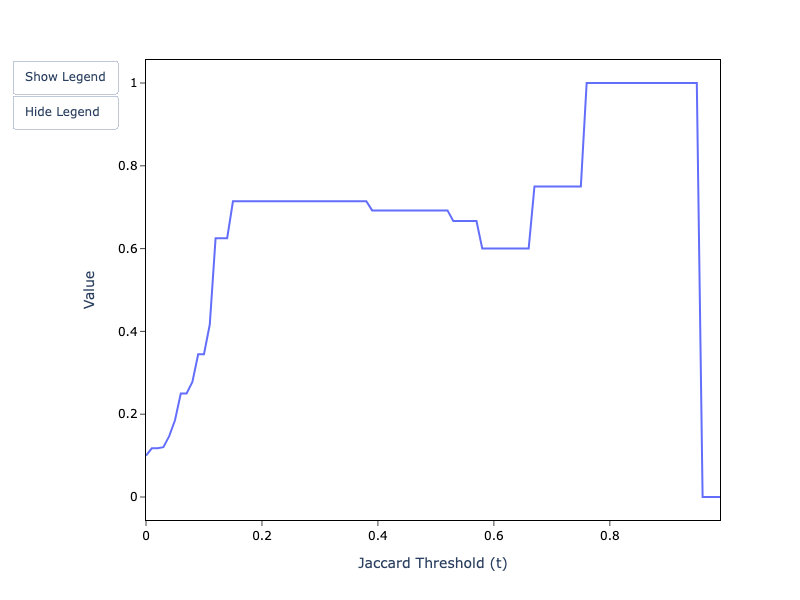
\includegraphics[width=\textwidth]{sample-usage/mini-fs-precision}
            \caption{F-S Precision}
        \end{minipage}    
        \begin{minipage}{0.32\textwidth}
            \centering
            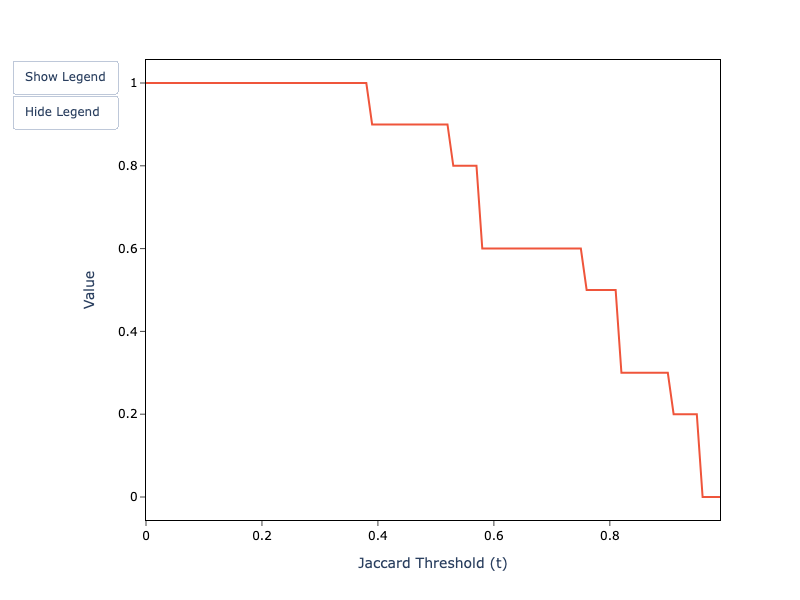
\includegraphics[width=\textwidth]{sample-usage/mini-fs-recall}
            \caption{F-S Recall}
        \end{minipage}    
        \begin{minipage}{0.32\textwidth}
            \centering
            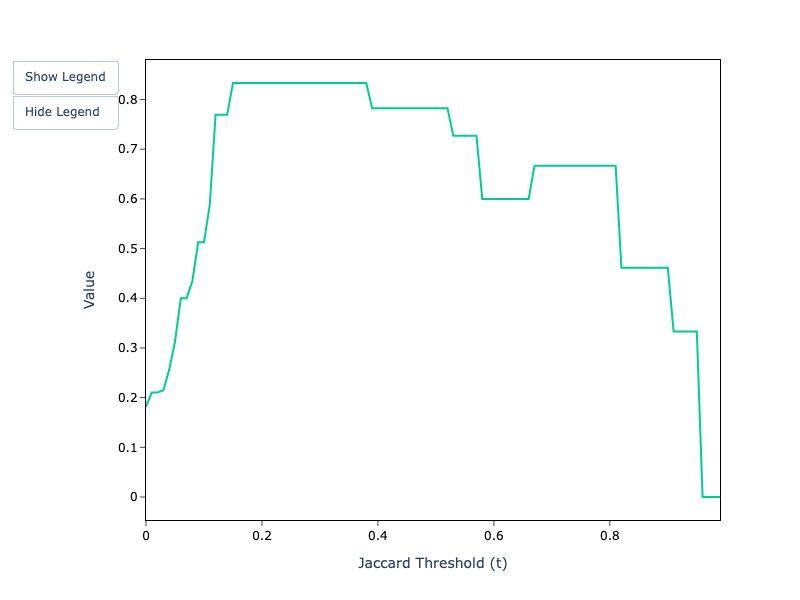
\includegraphics[width=\textwidth]{sample-usage/mini-fs-f1}
            \caption{F-S F1}
        \end{minipage}
    \end{figure*}
    \begin{figure*}
        \begin{minipage}{0.32\textwidth}
            \centering
            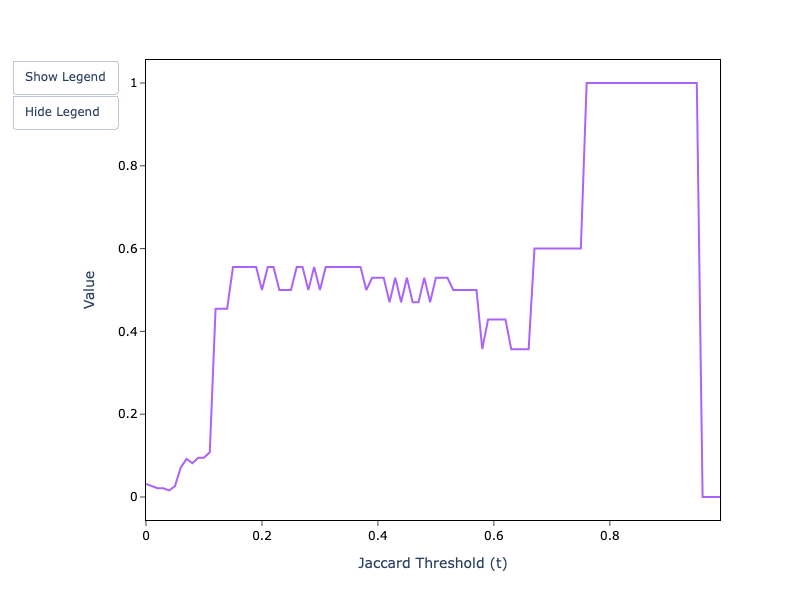
\includegraphics[width=\textwidth]{sample-usage/mini-alg-pp}
            \caption{Pairwise Precision}
        \end{minipage}    
        \begin{minipage}{0.32\textwidth}
            \centering
            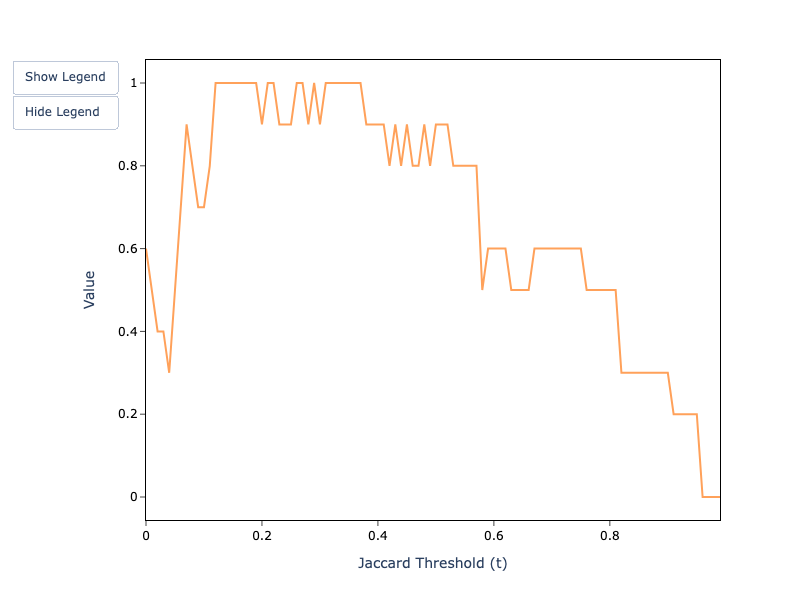
\includegraphics[width=\textwidth]{sample-usage/mini-alg-pr}
            \caption{Pairwise Recall}
        \end{minipage}    
        \begin{minipage}{0.32\textwidth}
            \centering
            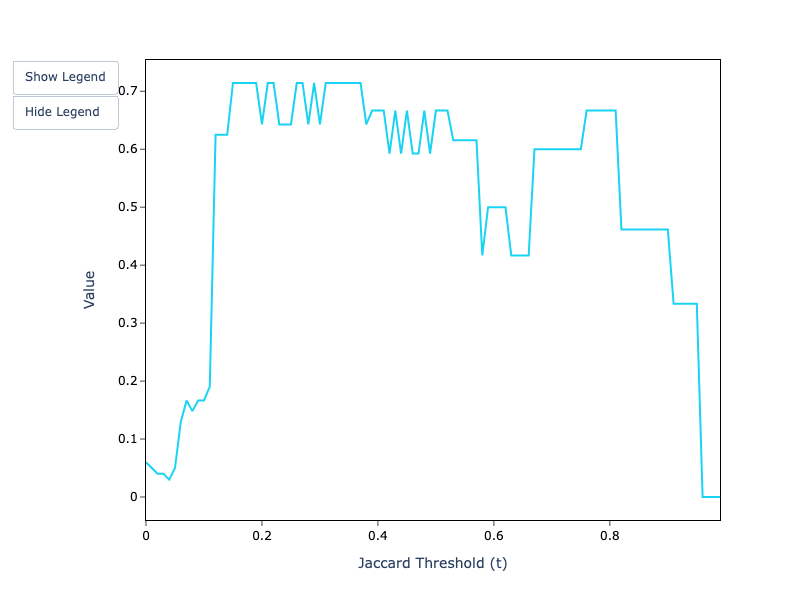
\includegraphics[width=\textwidth]{sample-usage/mini-alg-pf}
            \caption{Pairwise F Measure}
        \end{minipage}
    \end{figure*}
    \begin{figure*}
        \begin{minipage}{0.32\textwidth}
            \centering
            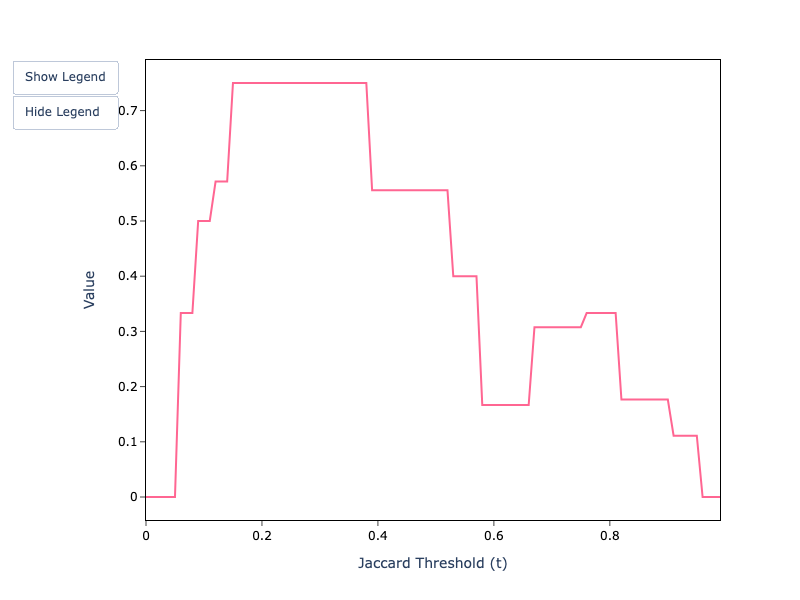
\includegraphics[width=\textwidth]{sample-usage/mini-alg-cp}
            \caption{Cluster Precision}
        \end{minipage}    
        \begin{minipage}{0.32\textwidth}
            \centering
            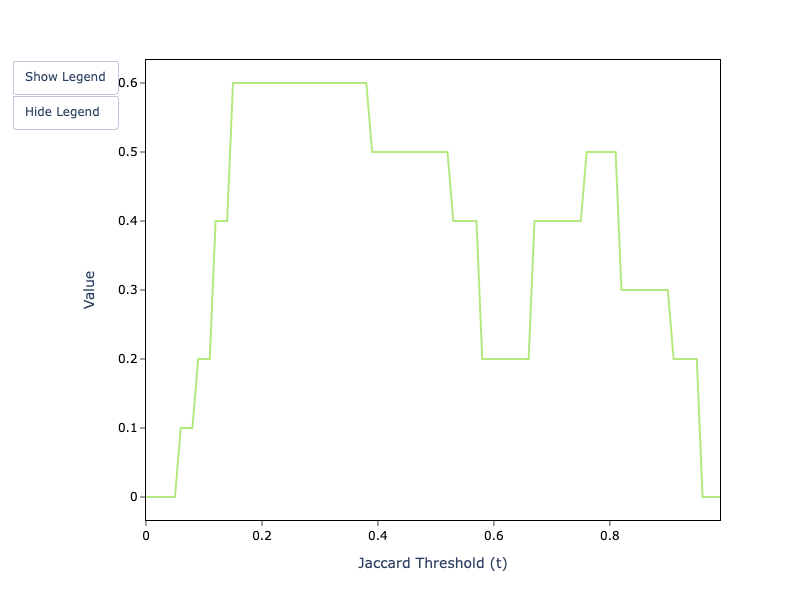
\includegraphics[width=\textwidth]{sample-usage/mini-alg-cr}
            \caption{Cluster Recall}
        \end{minipage}    
        \begin{minipage}{0.32\textwidth}
            \centering
            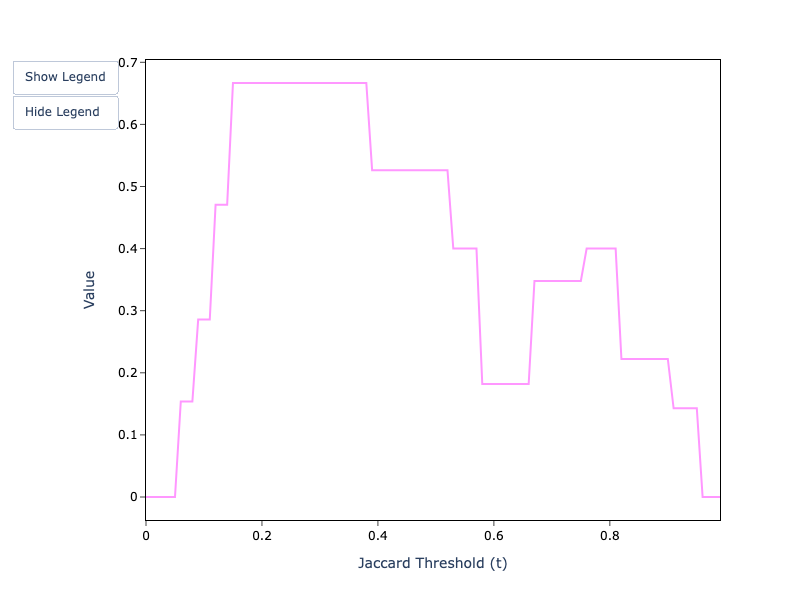
\includegraphics[width=\textwidth]{sample-usage/mini-alg-cf}
            \caption{Cluster F Measure}
        \end{minipage}
    \end{figure*}
    \begin{figure*}[h!]
        \begin{minipage}{0.32\textwidth}
            \centering
            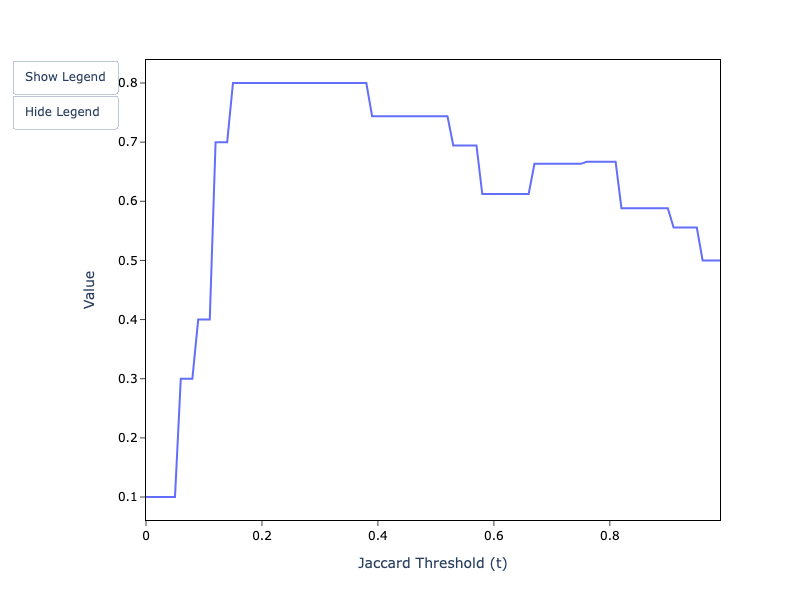
\includegraphics[width=\textwidth]{sample-usage/mini-alg-twi}
            \caption{Talburt-Wang Index}
        \end{minipage}    
        \begin{minipage}{0.32\textwidth}
            \centering
            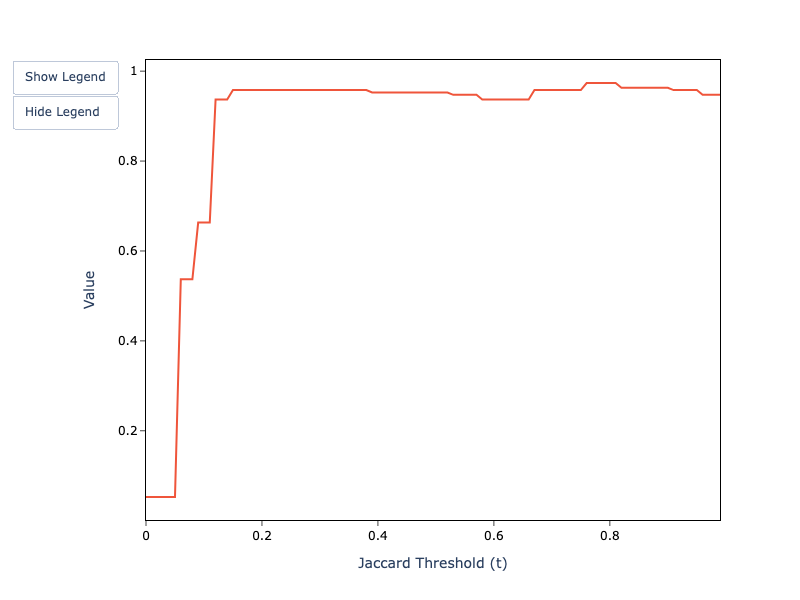
\includegraphics[width=\textwidth]{sample-usage/mini-alg-ri}
            \caption{Rand Index}
        \end{minipage}    
        \begin{minipage}{0.32\textwidth}
            \centering
            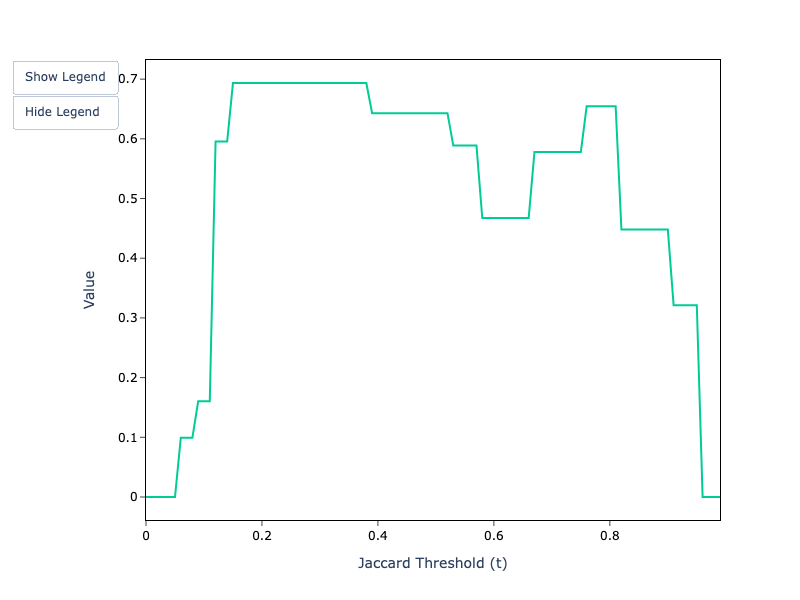
\includegraphics[width=\textwidth]{sample-usage/mini-alg-ari}
            \caption{Adjusted Rand Index}
        \end{minipage}
    \end{figure*}

    \subsection{Performance}

    Typically, we evaluate CPU performance in terms of throughput (for example
    millions of operations per second or MIPS).
    However ``comparing the MIPS of two different CPU architectures, such as
    Reduced Instruction Set Computers (RISCs) and Complex Instruction Set
    Computers (CISCs), is meaningless since the instructions on the two
    computers are unequal''\cite{jain1991profiling}.
    Since the introduction of a new generation of laptops by Apple, this concern
    is more present than ever.

    A concern that's similar to the one raised for CPU profiling can be raised
    about memory profiling in relation to the underlying operating system.
    Due to the variability of the outcomes during experimentation and the fact
    that all memory consumption is very dependent on the operating system and
    standard C library used for compiling and linking the Python interpreter,
    we found memory profiling not to provide great insights.

    Under these circumstances we have chosen to elaborate a method of profiling
    the CPU usage of the library which is agnostic to the underlying hardware.
    CPU profiling is useful in the context of judging the metrics provided by
    the library relatively to one another.
    Our goal is to provide enough information so that by corroborating this
    information with our previous sample we gain a good idea about which metric
    supported by the library to use under which circumstances.
    
    For our CPU profiling session, we run the PPJoin algorithm over the same
    dataset as in the previous experiment and store the results in a file
    along with the ground truth.
    In our sample application for this experiment, we load the results and 
    ground truth from the file and run all of the Fellegi-Sunter and algebraic
    metrics while profiling the CPU usage.
    We have broken down the experiment into two steps to prevent running the
    entity resolution task from interefering with collecting the CPU profiling
    data.

    We use flamegraphs\cite{flamegraphs2013} to represent the CPU usage
    patterns in the library and the \texttt{cProfile} package from the Python
    standard library to trace the execution of the functions that compute
    metrics.

    \begin{figure*}[h!]
        \centering
        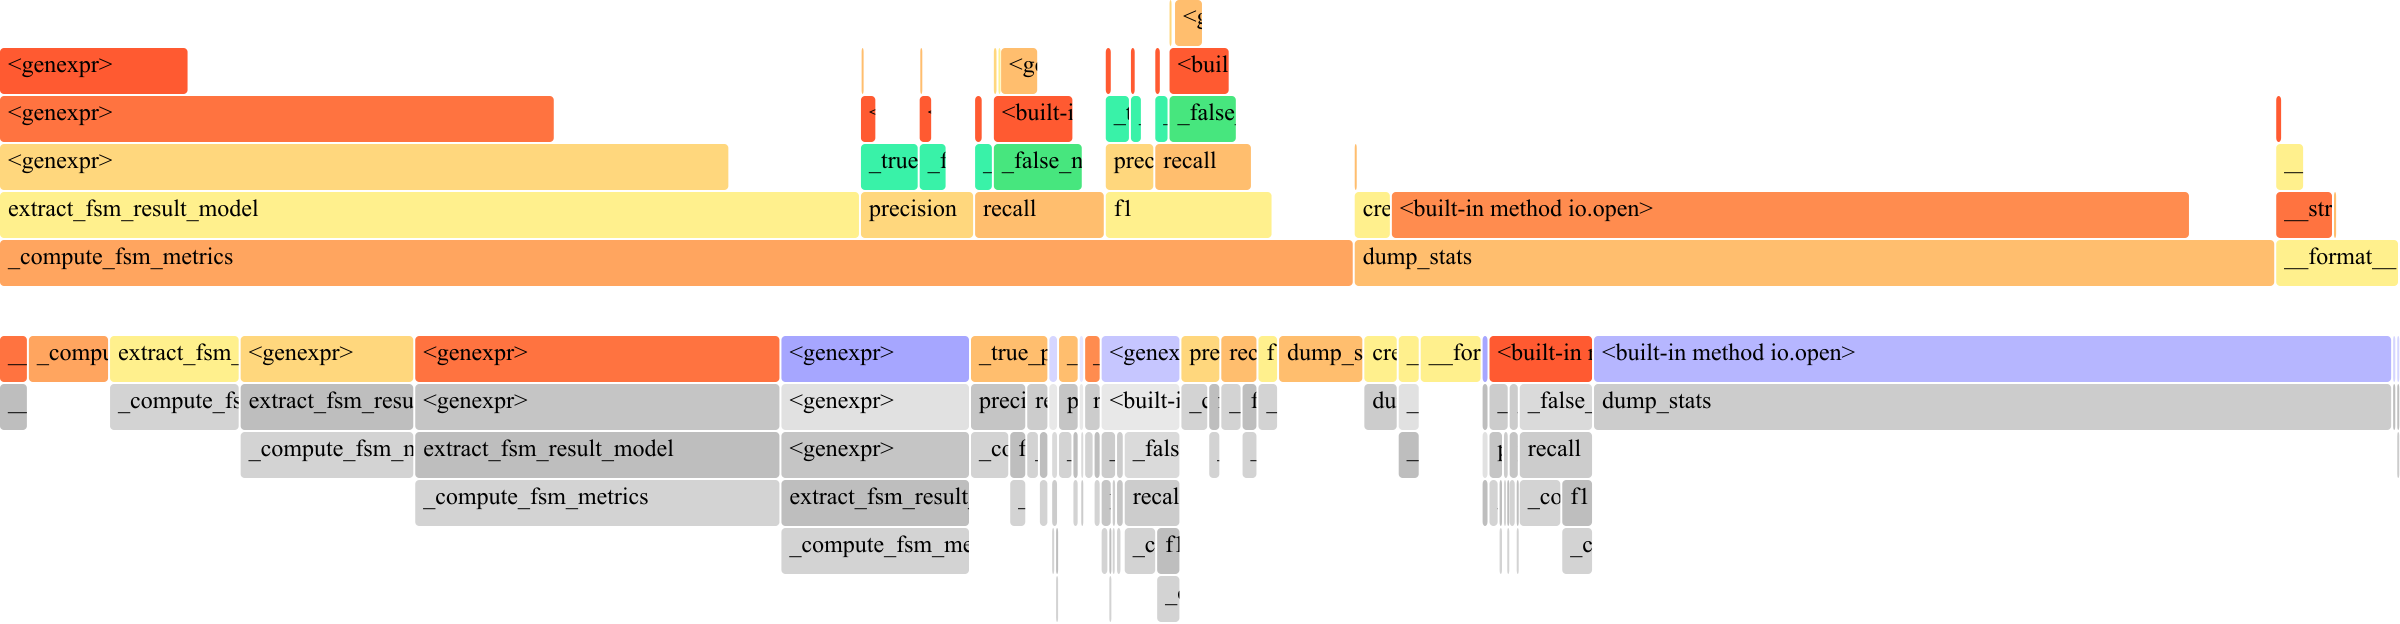
\includegraphics[width=\textwidth]{performance/fs-flamegraph}
        \caption{Fellegi-Sunter CPU Performance}\label{fig:fs-cpu-perf}
    \end{figure*}

    The flame graph in Figure~\ref{fig:fs-cpu-perf}
    shows that the Fellegi-Sunter metrics take up less CPU than the validation
    of the input and output of data.
    The main consumers are shown in Table~\ref{table:fs-cpu-perf}
    
    \begin{table*}[ht!]
        \centering
        \begin{tabular}{||c c c c||}
            \hline
            Metric & Cumulative Time & Number of Calls & Time per Call \\ [0.5ex]
            \hline\hline
            \texttt{recall} & 7.208e-06 & 2 & 3.604e-06 \\
            \hline
            \texttt{f1} & 5.291e-06 & 1 & 5.291e-06 \\
            \hline
            \texttt{precision} & 4.75e-06 & 2 & 2.375e-06 \\
            \hline
        \end{tabular}
        \caption{Fellegi-Sunter Metrics}
        \label{table:fs-cpu-perf}
    \end{table*}

    The best lesson we can learn here is that computing the statistical metrics
    is not resource-intensive at all.

    \begin{figure*}[h!]
        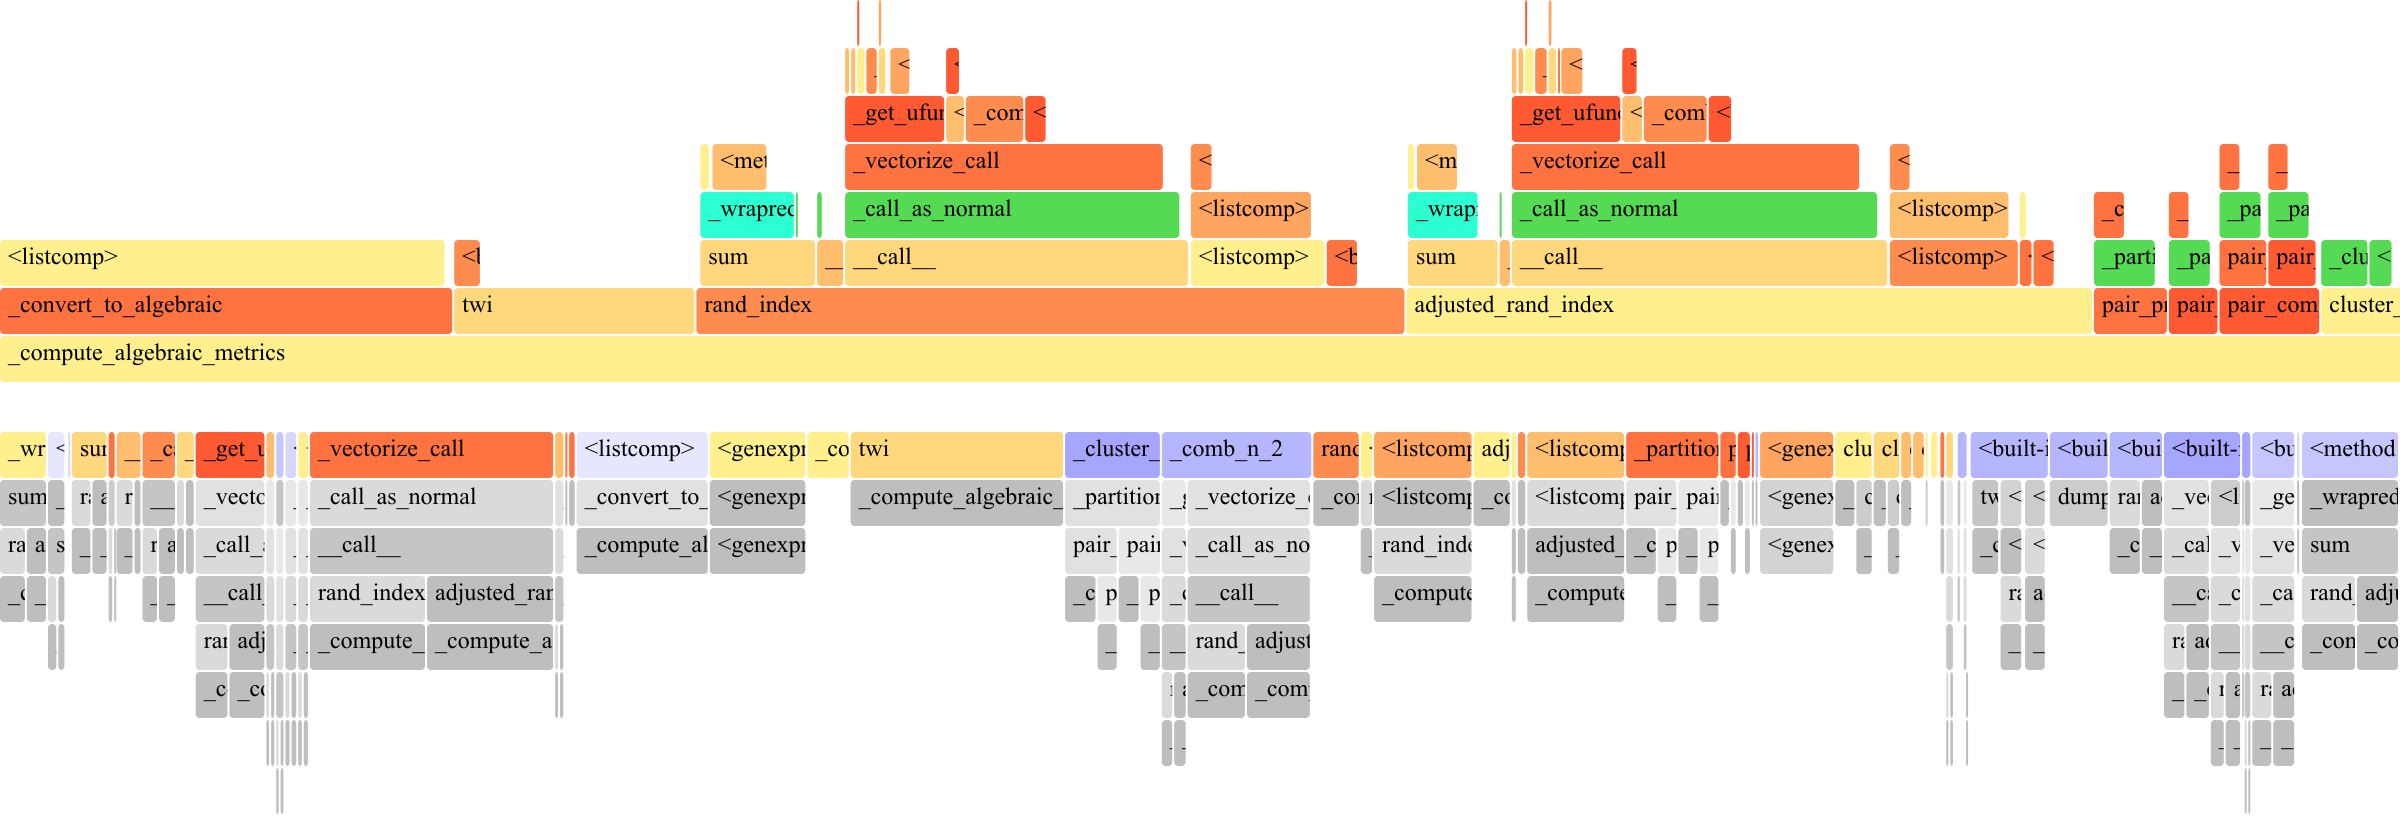
\includegraphics[width=\textwidth]{performance/algebraic-flamegraph}
        \caption{Algebraic CPU Performance}\label{fig:alg-cpu-perf}
    \end{figure*}
    
    The same cannot be said about the metrics that work with partitions over an
    input set.
    Table~\ref{table:alg-cpu-perf} presents how the algebraic metrics perform.

    \begin{table*}[ht!]
        \centering
        \begin{tabular}{||c c c c||}
            \hline
            Metric & Cumulative Time & Number of Calls & Time per Call \\ [0.5ex]
            \hline\hline
            \texttt{rand\char`_index} & 0.0004027 & 1 & 0.0004027 \\
            \hline
            \texttt{adjusted\char`_rand\char`_index} & 0.0001944 & 1 & 0.0001944 \\
            \hline
            \texttt{twi} & 9.146e-05 & 1 & 9.146e-05 \\
            \hline
            \texttt{cluster\char`_comparison\char`_measure} & 5.35e-05 & 1 & 5.35e-05 \\
            \hline
            \texttt{cluster\char`_recall} & 5.154e-05 & 2 & 2.577e-05 \\
            \hline
            \texttt{cluster\char`_precision} & 4.271e-05 & 2 & 2.135e-05 \\
            \hline
            \texttt{pair\char`_precision} & 2.971e-05 & 2 & 1.485e-05 \\
            \hline
            \texttt{pair\char`_recall} & 2.613e-05 & 2 & 1.306e-05 \\
            \hline
            \texttt{pair\char`_comparison\char`_measure} & 2.596e-05 & 1 & 2.596e-05 \\
            \hline
        \end{tabular}
        \caption{Algebraic Metrics}
        \label{table:alg-cpu-perf}
    \end{table*}

    The pairwise and cluster metrics still perform well as indicated in
    Figure~\ref{fig:alg-cpu-perf}.
    However, when we move on to consider the performance of the three supported
    indices, we see that computing the Rand Index and the Adjusted Rand Index
    prove to be the most onerous operations by far.

    We take note that the \texttt{\char`_convert\char`_to\char`_algebraic}
    function that checks whether the metrics are applied to two partitions over
    the same set is also a large consumer of CPU time.
    However, since that function is executed nine times (once for computing each
    metric) we declare ourselves content to file a note to improve the
    performance of that function at a later time.

    Perhaps the most important lesson to learn here is that algebraic metrics
    are an order of magnitude more expensive to compute than statistical
    metrics with this library.
    Moreover, not all algebraic metrics were created equal: the rand indexes
    are an order of magnitude more expensive to compute than the other metrics.
    Therefore, because the Talburt-Wang index seems to approximate the Rand
    index well enough, it might be a preferable choice to measure how well an
    entity resolution algorithm performs clustering.

    \section{Conclusions and Future Work}\label{sec:conclusions_and_future}

    \subsection{Conclusions}

    We have introduced a library for evaluating entity resolution results that
    is based on standards and Python protocols, making it highly interoperable.
    The application programming interface exposed by this library is deeply
    rooted in the mathematical models fundamental to entity resolution.
    By doing so the library ensures that data is represented in a way that is
    specific to entity resolution and not specific to another scientific problem
    or to a particular entity resolution system or task.
    Working with pairs or groups of entity references instead of labeling
    data should provide a much more user-friendly experience.

    The performance of the library is sound because it externalizes
    computationally expensive tasks to native code.
    The accuracy of the implemented metrics is verified automatically through
    unit tests.

    These attributes render the library not only highly beneficial but also low
    maintenance, making it an invaluable asset for all those passionate about
    entity resolution.

    \subsection{Missing Metrics}

    The entity resolution models we have touched upon so far support many more
    metrics that the library does not currently implement.
    Hitesh et al provide an insightful overview\cite{hitesh2012}.
    For well-rounded support of the models mentioned so far, the library would
    need to implement at least:
    \begin{itemize}
        \item additional cluster comparisons, such as the Closest Cluster $F_1$, the
        MUC $F_1$, $B^3 F_1$ and the $CEAF F_1$\cite{hitesh2012}
        \item additional Rand-like indexes\cite{warrens2022understanding}
    \end{itemize}

    \subsection{Missing Models}

    Besides the models we have covered herein, entity resolution has been
    theorized to be a graph problem\cite{eager2021} or an exercise in lattice
    theory with an ordering relation based on
    ``merge dominance''\cite{Ben2009Swoosh}.
    The mathematical model foundational to entity resolution significantly
    influences the data structures employed in implementing metrics that
    evaluate the quality of an entity resolution task within that model.
    More work is required to distil the data structures and the metrics we can
    use to evaluate entity resolution tasks using those models.

    New models might also bring to light new interesting metrics to
    measure the performance of entity resolution tasks.
    Variation of information\cite{meila2007vi} and the generalized merge
    distance\cite{Men10} are two examples of distance-based metrics for entity
    that we would like to implement.

    \bibliographystyle{apalike}
    {
        \small
        \bibliography{er-general,er-related-work,er-additional-references,er-software}
    }
\end{document}
